\usepackage{tikz}
\usepackage{eso-pic}
\usepackage{fancyhdr}
\usepackage{fontawesome5}
\usepackage{xurl}
\definecolor{MSPAzul}{HTML}{003872}
\definecolor{MSPTurquesa}{HTML}{008A99}
\definecolor{Cuadricula}{HTML}{E4EDF4}
\AddToShipoutPictureBG{\begin{tikzpicture}[remember picture,overlay]\draw[step=5mm,Cuadricula,line width=0.12pt](current page.south west) grid (current page.north east);\end{tikzpicture}}
\pagestyle{fancy}\fancyhf{}
\fancyhead[L]{
\includegraphics[width=5.8cm]{recursos/logo_msp.png}}\fancyhead[R]{
\includegraphics[width=1.8cm]{recursos/banco_mundial.png}}
\renewcommand{\headrulewidth}{0.35pt}\renewcommand{\footrulewidth}{0.2pt}
\newcommand{\PieContacto}{\parbox[b]{0.62\textwidth}{\raggedright\fontsize{7.2}{9}\selectfont
  Marcelo Chávez\\[-1pt]
  Consultor Especialista en Protección Social - Banco Mundial\\[-1pt]
  \textcolor{MSPAzul}{\faEnvelope\enspace marcelo\_chavez\_ec@outlook.com\quad
  \faIcon{mobile-alt}\enspace 0983332687\quad \faLinkedin}}}
\fancyfoot[L]{\PieContacto}
\fancyfoot[R]{\parbox[b]{0.38\textwidth}{\raggedleft\fontsize{6.8}{8.5}\selectfont \mbox{Manual de usuario de SIGEM}\\[-1pt]página \thepage}}
\fancypagestyle{plain}{\fancyhf{}\fancyhead[L]{
\includegraphics[width=5.8cm]{recursos/logo_msp.png}}\fancyhead[R]{
\includegraphics[width=1.8cm]{recursos/banco_mundial.png}}\fancyfoot[L]{\PieContacto}\fancyfoot[R]{\parbox[b]{0.38\textwidth}{\raggedleft\fontsize{6.8}{8.5}\selectfont \mbox{Manual de usuario de SIGEM}\\[-1pt]página \thepage}}}
\setlength{\footskip}{42pt}
\setkomafont{chapter}{\normalfont\LARGE\bfseries\color{MSPAzul}}
\setkomafont{section}{\normalfont\large\bfseries\color{MSPAzul}}
\setkomafont{subsection}{\normalfont\normalsize\bfseries\color{MSPAzul}}
\setlength{\parskip}{4pt}\setlength{\emergencystretch}{3em}
\renewcommand{\maketitle}{\begin{titlepage}\thispagestyle{empty}\noindent
\includegraphics[width=6.8cm]{recursos/logo_msp.png}\hfill
\includegraphics[width=2cm]{recursos/banco_mundial.png}\par\vspace*{35mm}\begin{center}{\color{MSPAzul}\fontsize{28}{34}\selectfont\bfseries Manual de usuario de SIGEM\par}\vspace{8mm}{\color{MSPTurquesa}\large Sistema Institucional de Gestión y Monitoreo\par}\vspace{12mm}{\large Ministerio de Salud Pública\par}\end{center}\vfill\begin{flushleft}{\small Versión revisada: 3 de noviembre de 2026\par}\end{flushleft}\end{titlepage}}
